\documentclass[12pt,a4paper]{article}
\usepackage[
	left 	= 2.5cm,
	right 	= 2.5cm, 
	top 		= 2.5cm,
	bottom 	= 2.5cm,
]{geometry}
\usepackage[utf8]{inputenc}
\usepackage[english]{babel}
\usepackage[OT1]{fontenc}
\usepackage{amsmath}
\usepackage{mathtools}
\usepackage{graphicx}
\usepackage{caption}
\usepackage[round]{natbib}

\usepackage[hidelinks]{hyperref}
\hypersetup{
	colorlinks = true,
	urlcolor   = blue,
	linkcolor  = black, 
	citecolor  = blue, 
}


\usepackage{fancyhdr}
\pagestyle{fancy}


\usepackage{titlesec,xcolor}
\titleformat{\section}{\bfseries}{\thesection}{0.5em}{}
\titlespacing{\section}{0pt}{3ex plus 1ex minus 0.2ex}{10pt}
\setlength{\headheight}{14.49998pt}

\usepackage{titlesec,xcolor}
\titleformat{\subsection}{\bfseries}{\thesubsection}{0.5em}{}
\titlespacing{\subsection}{0pt}{3ex plus 1ex minus 0.2ex}{10pt}
\setlength{\headheight}{14.49998pt}


%------------------------------------------------------------------%

\author{Lucas Paul Unterweger, Sophia Oberbrinkmann, Fynn Lohre}
\title{The Kremlin Effect: How Geographical Proximity to Russia Affects Military Spending}


\begin{document}

\begin{titlepage}
\center
\vfill

\includegraphics[scale=0.08]{WU.png}
\vfill
\begin{tabular}[t]{lc}
Course:  & Advanced Macroeconometrics (Science Track) \\
Examiner: & 
Nikolas Kuschnig, MSc (WU) \& Lukas Vashold, MSc (WU) \\
Submission date: & 30.09.2023 \\
\end{tabular}
\vfill
{\large \textbf{The Kremlin Effect: How Geographical Proximity to Russia Affects Military Spending}}
\vfill
by\\ \vspace{3mm}
{\Large Fynn Lohre \href{https://github.com/VARFynn}{
\includegraphics[scale=0.01]{GitHub.png}}}\\
(Matr.-Nr. h12232560)\\ \vspace{3mm}
\& \\ \vspace{3mm}
{\Large Sophia Oberbrinkmann \href{https://github.com/SophiaOberbrinkmann}{
\includegraphics[scale=0.01]{GitHub.png}}}\\
(Matr.-Nr. h12225352)\\ \vspace{3mm}
\& \\ \vspace{3mm}
{\Large Lucas Unterweger \href{https://github.com/therealLucasPaul}{
\includegraphics[scale=0.01]{GitHub.png}}}\\
(Matr.-Nr. h11913169 )\\ \vspace{3mm}
\vfill

\thispagestyle{empty}
\pagebreak
\end{titlepage}
\newcounter{savepage}
\pagenumbering{roman}
\thispagestyle{empty}
\begin{abstract}
\textit{We present a study on how the distance of a country’s capital to Moscow affects its military spending. To tackle the research question, we combine different datasets from various sources, such as the SIPRI Military Expenditure Database, the GeoDist database, and the Electoral Democracy Index. A Bayesian Model Averaging (BMA) approach is used to account for model uncertainty and estimate several models with different distance measures and covariates. Our results identify a in terms of posterior model probability superior model and show that the capital distance to Moscow has a significant negative effect on military expenditures, implying that countries closer to Russia perceive a higher threat and allocate more resources to defense. Additionally, it's observable that continents play a pivotal role in explaining the variation in military expenditures. Specifically, a general underestimation of possible threats in Europe is indicated. The effects of border degree and democracy index as additional layers of distance are mixed and remain to some extend uncertain.} 
\end{abstract}
\clearpage
\thispagestyle{plain}
\tableofcontents
\pagebreak
\setcounter{savepage}{\arabic{page}}
\pagenumbering{arabic}
\section{Introduction}

Our research project delves into the intriguing question of whether the distance of a country's capital to Moscow has a significant impact on its military expenditure. To tackle this question, we employ a Bayesian regression analysis.\\

The research is inspired and built upon the insights provided by two seminal papers: the work of Kofron and Stauber (2023) and Nordhaus et al. (2012). Kofron and Stauber (2023) focused on the Russo-Ukrainian conflict's impact on the military expenditures of European States. They made a thought-provoking observation, suggesting that physical geography continues to play a pivotal role in shaping military affairs and geopolitics, even in the 21st century. On the other hand, Nordhaus et al. (2012) investigated how a country's external security environment influences its military spending. Their extensive analysis, covering 165 countries from 1950 to 2000, demonstrated that the prospectively generated estimate of the external threat served as a potent variable in explaining military expenditures. Drawing upon these foundational ideas, our research seeks to utilize the geographical distance to Russia, as highlighted by Kofron and Stauber (2023), as a proxy for external threat, echoing Nordhaus's emphasis. To justify this assumption, we consider the historical background of Russia and the Soviet Union. Given that the NATO was established as a response to the perceived political aggression of the Soviet Union during the Cold War, and it currently comprises 31 member states, it reinforces our belief that Russia is often seen as a potential threat.\\

While our focus centers on the geographical distance to Russia as an external factor influencing military expenditure, we recognize that numerous other determinants have been extensively analyzed. A plethora of authors have shed light on different potential "causes", broadly categorized into external factors (such as military expenditures of potential enemies or allies, and perceived threats) and internal influences, encompassing economic, political, and bureaucratic factors (Nikolaidou (2008)). The research results across various studies, some conducted on individual countries while others on groups of countries or spanning the entire globe (Nikolaidou (2008), George (2018) and Nordhaus et al. (2012)), have yielded somewhat ambiguous findings (Nikolaidou (2008), Odenhal(2020)). 
Given the relative dearth of studies exploring the specific influence of geographical distance to Russia on military spending (Kofron and Stauber (2023)), we aim to contribute to the existing literature by focusing on this understudied factor. Our expectation is that a closer distance to Russia would be positively correlated with increased military expenditure by the concerned country. \\ 

As part of our investigation, we also consider the NATO member countries, who are expected to allocate 2 \% of their annual GDP to military expenditures uniformly. Any deviation from this standard percentage rate could further strengthen our hypothesis, as one reason from this deviation might be the influence of the geographical distance to Russia. Furthermore, we expand our analysis beyond NATO members to include non-NATO countries, recognizing that recent events like the Russo-Ukraine conflict highlight Russia's perceived threat by countries worldwide. Our study encompasses a total of 147 countries, offering a comprehensive global perspective. \\

To gauge the geographical distance to Russia, we explore various approaches, evaluating how the estimation may be influenced by these different measures. Our primary proxies are the capital distances of countries measured in kilometers, as this offers an appropriate metric for military threats. While Kofron and Stauber (2023) considered road travel distance and mention the potential of flight travel distance, we focus on air distance as a proxy when examining military threats. 
In our pursuit of a comprehensive and nuanced analysis, we recognize that relying solely on the distance between capitals might not fully capture the complex dynamics and interactions between countries. Therefore, we go beyond the capital distance and incorporate a second measure — the border degree of a country with Russia — to gain deeper insights into the relationship between geographical proximity and military expenditure decisions. The border degree metric enables us to examine how the presence of a common border with Russia, or even a second-degree border (i.e., sharing a border with a country that shares a border with Russia), may exert distinct influences on a country's military spending compared to the air distance metric. By exploring the border degree, we aim to understand whether physical contiguity with Russia plays a unique role in shaping a country's perception of threats and security concerns, and consequently, its military expenditure decisions. Countries sharing a direct border with Russia may experience more immediate security considerations, influenced by historical conflicts, geopolitical tensions, or territorial disputes. On the other hand, second-degree border countries might have indirect security implications resulting from their proximity to nations with a direct border with Russia. These indirect influences might manifest in different ways and warrant closer examination.\\

Moving forward, our research report will be structured as follows: we will first delve into the \textit{Econometric Framework}, with particular emphasis on our novel approach of employing Bayesian Model Averaging, a technique not previously utilized in the papers we draw inspiration from. Subsequently, we will detail the \textit{Data and Variables}, we utilize, emphasizing its relevance and reliability. We will then present the \textit{Results} of our investigation, providing insights into the potential relationships uncovered, before we analyze the prevailing \textit{Implications} and \textit{Limitations}   in the \textit{Discussion}. Finally, we will conclude the project with a comprehensive \emph{Conclusion}, highlighting the implications of our findings and potential avenues for further research.

\section{Econometric Framework}
In order to draw meaningful conclusions while acknowledging the potential uncertainty in our models, we have adopted Bayesian Model Averaging (BMA) as our approach to address our core research question. BMA effectively accommodates model uncertainty by simultaneously considering multiple competing models. In empirical research, it’s often the case that there is substantial uncertainty about the appropriate model specification. Model uncertainty arises due to the abundance of existing theories or available control variables (as discussed by Steel (2020)). It becomes particularly pronounced when there is a multitude of potential models to choose from, and the determination of the “best” model is not straightforward. When dealing with a specific endogenous variable and a set of possible predictors, the issue of variable selection becomes a central concern (see Clyde and George (2004)). \\

In the context of understanding the determinants of military expenditure, there are numerous factors beyond proximity to Russia that might influence or correlate with military spending. This introduces the challenges of model uncertainty. The extensive body of existing literature addressing various aspects of this issue underscores the problem’s complexity. For instance, Nordhaus et al. (2012) investigate how a country’s external security environment affects its military spending, considering variables like real GDP, the weighted military expenditures of friendly and hostile nations, democracy scores, and the estimated annual probability of a significant civil conflict as control variables. On the other hand, Kofron and Stauber (2023) focus on geographical distance as a potential driver of military expenditure and incorporate several variables as controls, including the number of terrorist attacks, government ideology, GDP growth, and historical factors like post-communism and the presence of Soviet military forces. \\

Economic growth is the central theme in many studies on military expenditure, and Lin and Wang’s 2019 literature review demonstrate the ambiguous findings in this regard. Furthermore, Albelate, Bel and Elias (2009) delve into the institutional determinants of military spending, emphasizing the general observation that democracies tend to allocate less to defense than autocracies, while also scrutinizing specific democratic systems. Dunne and Perlo-Freeman (2003a and b), as well as Nikolaidou (2008) focus on economic, political, and strategic factors. It is worth noting that Dunne and Perlo-Freeman highlight changes in determinants of military expenditure following the Cold War. A myriad of other studies has explored various facts of this topic, but we won’t delve into them here. For a general literature review, see Albeta, Bel and Elias (2009). \\

The existing body of literature on the determinants of military expenditure underscores the presence of model uncertainty. To address this uncertainty, we have chosen the Bayesian Model Averaging (BMA) approach. Instead of merely estimating a single model $\hat{M}$ and updating our prior belief $p(\theta)$ to posterior beliefs $p(\theta \vert data)$, we consider all the models within the model space under consideration. We then compute an average across these models to find possible driving foreces of the military expenditure decision making or correlation. This approach considers the diversity of models $M_{i}$, allowing for variation and differences between them. We derive a combined parameter distribution, weighted by the posterior model probabilities of all models within the model space, to draw our conclusions. These posterior model probabilities reflect the plausibility of a given model based on the data, denoted as $p(M_{i}\vert data)$, following the BMA methodology as outlined by Steel (2020), Brown et al. (2002),  Hoeting et al. (1999) and Moral-Benito (2015).\\

To implement BMA, we employ the “BMA” package within the R programming environment, utilizing the “bicreg” function. When the number of covariates is fewer then 30, the BMA package exhaustively considers all possible models. It’s important to note that the BMA package has limited flexibility when it comes to model priors, assuming equal a priori treatment for all models. Regarding the prior for regression coefficients, we anticipate that the BMA approach is sensitve to the prior choice, but the used BMA package is again inflexible in this rgard and relies on the Bayesian Information Criterion (BIC) approximation, which closely resembles the Unit Information Prior (Amini and Parmeter (2011)). To compare and evaluate competing models, we utilize the Bayesian Information Criterion (BIC) and posterior probabilities. The optimal model is selected based on having the lowest BIC value and the highest posterior probability (Starkweather (2011)).


\section{Data and Variables}
For the purpose of this paper, we combine different datasets. Our dependent variable "pct" is defined as the ”Military Expenditure by Country as percentage of GDP”. We use the SIPRI Military Expenditure Database (2023) by the Stockholm International Peace Research Institute (SIRPI). Their definition of military expenditure includes all spending on current military forces and activities, meaning the armed forces, including peace keeping forces; defense ministries and other government agencies engaged in defense projects; paramilitary forces, when used to be trained, equipped and available for military operations; and military space activities. With respect to the reliability of the data, it should be noted that the data collected is not only derived from primary sources, but also includes secondary sources and estimates, e.g., by the IMF or NATO. \\

Our primary variable, the capital distances to Russia “dist”, is taken from the CEPII database. The GeoDist database is provided by the \textit{Centre d’Etudes Prospectives et d’Informations Internationales} (CEPII; Mayer and Zignago, 2011) and includes an exhaustive set of gravity variables. This engenders a bilateral measurement of distance, namely distance between the capital city in each country. For further information on the distance measure, we manually create dummy variables - Direct Border - and - Secondary Border -, capturing the existence of a direct border and a border with a state with a direct border, respectively.\\

Incorporating additional independent variables, we try to align with the hypotheses outlined in the previously mentioned literature. Kofron and Stauber (2023) put forward various hypotheses that informed their section of control variables. We intend to employ these hypotheses as a guiding framework for our own paper, helping us with the selection of appropriate control variables. We attempt to combine this approach with insights derived from other studies (Nordhaus et al. (2012), Lin and Wang (2019)). We use the variable “NATO” to signify, whether a state is a member of the NATO alliance. Building on Kofron and Stauber’s (2023) argument, which suggests that NATO member states tend to increase their military expenditure, we introduce an additional binary variable, which we label “OKVS”. This variable accounts for membership in the \textit{Collective Security Treaty Organization}. 
We introduce another variable “V-Dem”, which is supposed to represent the degree of democracy of a country. In doing so, we draw from the work of Albelate, Bel and Elias (2009), which explores institutional determinants of military spending, emphasizing the general observation that democracies tend to allocate less to defense than autocracies. The Electoral Democracy Index (V-Dem-Index) is based on the Varieties of Democracy (V-Dem) dataset (Coppedge et al., 2023) by the Department of Political Science located at the University of Gothenburg. The V-Dem Index categorizes countries along a scale from zero to one, indicating their degree of democracy. The democratic proximity is determined by calculating the difference between a country’s assigned value and that of Russia (approx. 0.22 depending on year). \\

Additionally, we incorporate two dummy variables: “BRICS”, which accounts for membership in the Collective Security Treaty Organization, and another dummy that captures political neutrality, using the world population review as a source of information. These two dummies are included to build upon the idea that political orientation can shape military expenditure, as explored by Kofron and Stauber (2023). While Kofron and Stauber used a more detailed measure based on the government political orientation, due to data availability constraints, we have condensed it to these two dummy variables. Kofron and Stauber (2023) furthermore state that: “States with historically strained relationship with Russia (USSR) will display bigger increases in their military spending” (p. 6). Thus, we introduce a dummy variable, controlling for former states belonging to the Soviet Union. As previously noted, there is an extensive body of literature exploring the relationship between military expenditure and economic growth. Lin and Wang (2019) point out, that "a number of studies have adressed the positive and negative correlations between military expenditure and economic growth" (p.3098) . In light of this, we incorporate the variable “GDP Growth” into our analysis. The variable is derived from the World Bank and represents the “GDP per capita growth (annual \% )”\\

In our analysis we focus exclusively on one specific year after 2001, as Gray (2005) claims it to be the end of the post-Cold War period (S.14). This leads to our final dataset which contains 147 countries after removing countries, that do not exist anymore, as well as Russia, Kosovo and South Sudan to derive our core data structure.

Recognizing that the variable "dist" remains constant over time, we opt for a cross-sectional regression approach. This method aligns with Buch's 2005 study, which examined the correlation between "dist" and international banking. In her analysis, Buch applied the gravity model and employed cross-sectional regression for each year within the period of 1983-1999. Given that this extensive time span is beyond the scope of our study, we narrow our focus to just one specific year, 2015. By doing so, we acknowledge that we will not account for changes over time, which would align with Buch's approach in 2005. For future investigations, it might be beneficial to consider a longitudinal analysis spanning multiple years. 

We will conduct Bayesian Model Averaging (BMA) using three different datasets: the entire dataset, a dataset comprising only NATO member countries, and another dataset consisting solely of EU member countries. This approach aims to determine if the selection of countries has any influence on the resulting outcomes. \\

 
\section{Results}
\subsection{Whole Dataset}

\begin{figure}[h]
\center
\label{F:2}
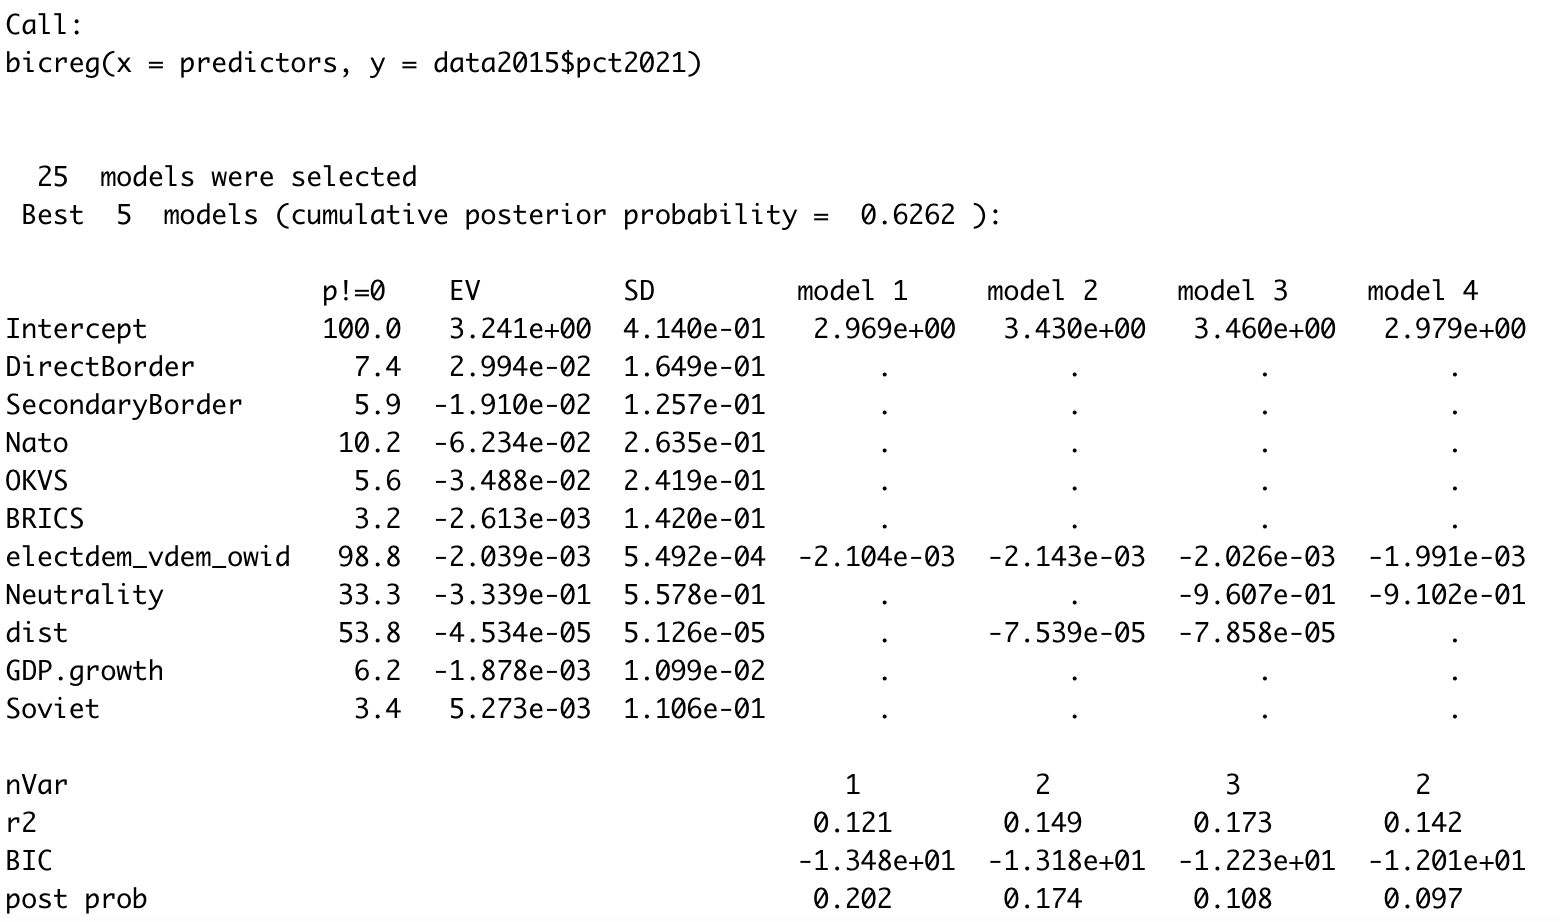
\includegraphics[scale=0.5]{BMA_results}
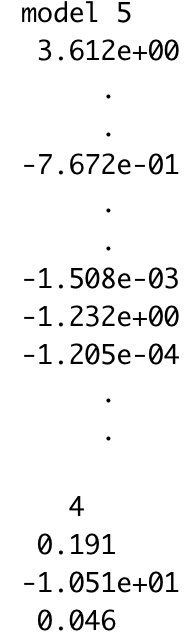
\includegraphics[scale=0.5]{BMA_results_2}
\caption{Bayesian Model Averaging - whole Data}
\end{figure}

In the output table (see Figure 1), the "p!=0" column signifies the probability that the coefficient for a given predictor is not zero among the 25 models that were generated. The "EV" column presents the Bayesian Model Averaging (BMA) posterior distribution mean for each coefficient, while the "SD" column displays the BMA posterior distribution standard deviation for each coefficient (Starkweather 2011). Only the five best models are presented here. \\

The initial model, "model 1", which includes only the variable "V-Dem", stands out as the best model in this context. It achieves this distinction by having the lowest Bayesian Information Criterion (BIC) score (-1.348e+1) and the highest posterior probability (0.202). Usually, the first model is expected to be the best, however, this might not always hold true, especially when theoretical considerations necessitate the inclusion of additional variables (Starkweather 2011). For this model, the coefficients for the "V-Dem" variable is -2.104e-03. Consequently, for every increse in the difference between a country's democracy index and that of Russia, there is a corresponding correlation to the country's military expenditure. Notable, neither of the distance variables are included in this model. 

In contrast, "model 2", which ranks second in terms of BIC (-1.348e+01) and posterior probability (0.174), introduces the variable "dist", measuring the air distance between a country's capital and Moscow. In this model, the coefficient for the distance is -7.539e-05. Here, an increase in the air distance of a country's capital to Moscow is correlated with a reduction in the expected military expenditure by the corresponding amount. The coefficient for the "V-Dem" variable in this model is -2.143e-03. Moving on to "model 3," it incorporates the "Neutrality" variable, which has a coefficient of -9.607e-01. Additionally, the distance variable in this model has the coefficient -7.858e-05 and the "V-Dem" Variable -2.026e-03. "Model 4" does not include the distance variable, but it still retains the "V-Dem" (-1.991e-03) and "Neutrality" (-1.991e-03) variables. Finally, Model 5 encompasses the most variables, including "NATO" (coefficient: -7.672e-01), "V-Dem" (-1.508e-03), "Neutrality" (-1.232e+00), and "distance" (-1.205e-04).\\

In Models 2, 3, and 5, the distance variable is one of the selected variables and the probability that the coefficient for the variable is not zero among the 25 models that were genertated is relatively high with 53.8\%. This suggests a correlation between a country's military expenditure and its distance from Russia. This supports our core reserach hypothesis. None of these models include the "Direct Border" and "Secondary Border" metrics. This is particularly surprising, as one would expect direct proximity to Russia to have an influence or correlate with the military expenditure of a country. One possible explanation could be that modern military conflicts, as anticipated by military spending, are not necessarily centered around annexation and territorial disputes. Another hypothesis could be that the impact of modern weapon systems is less dependent on direct border contact than traditional trench warfare conflicts.

The "V-Dem" variable, which measures the difference in a country's democracy index compared to that of Russia, is included in all five suggested models and has a probability of 98.8\% that the coefficient is not zero among the generated models. One hypothesis could be that a country's institutional situation compared to that of Russia serves as a "political distance." Increased differences in a country's institutional situation compared to Russia could positively correlate with higher military expenditure.

The dummy variables "OKSV" and "BRICS," which measure membership in these alliances, are not included in any of the suggested models, possibly, because these measures might be too weak to be considered as variables measuring the political orientation of a country. Furthermore, the "GDP growth" variable is absent in all of the models under consideration, which is not in line with the broad literature dealing with this topic. This could be explained by the choice of a cross-sectional analysis instead of a time-series analysis, as a change over a larger time period could have a bigger impact than the consideration of just one year.  \\


\subsection{NATO members}
\begin{figure}[h]
\center
\label{F:2}
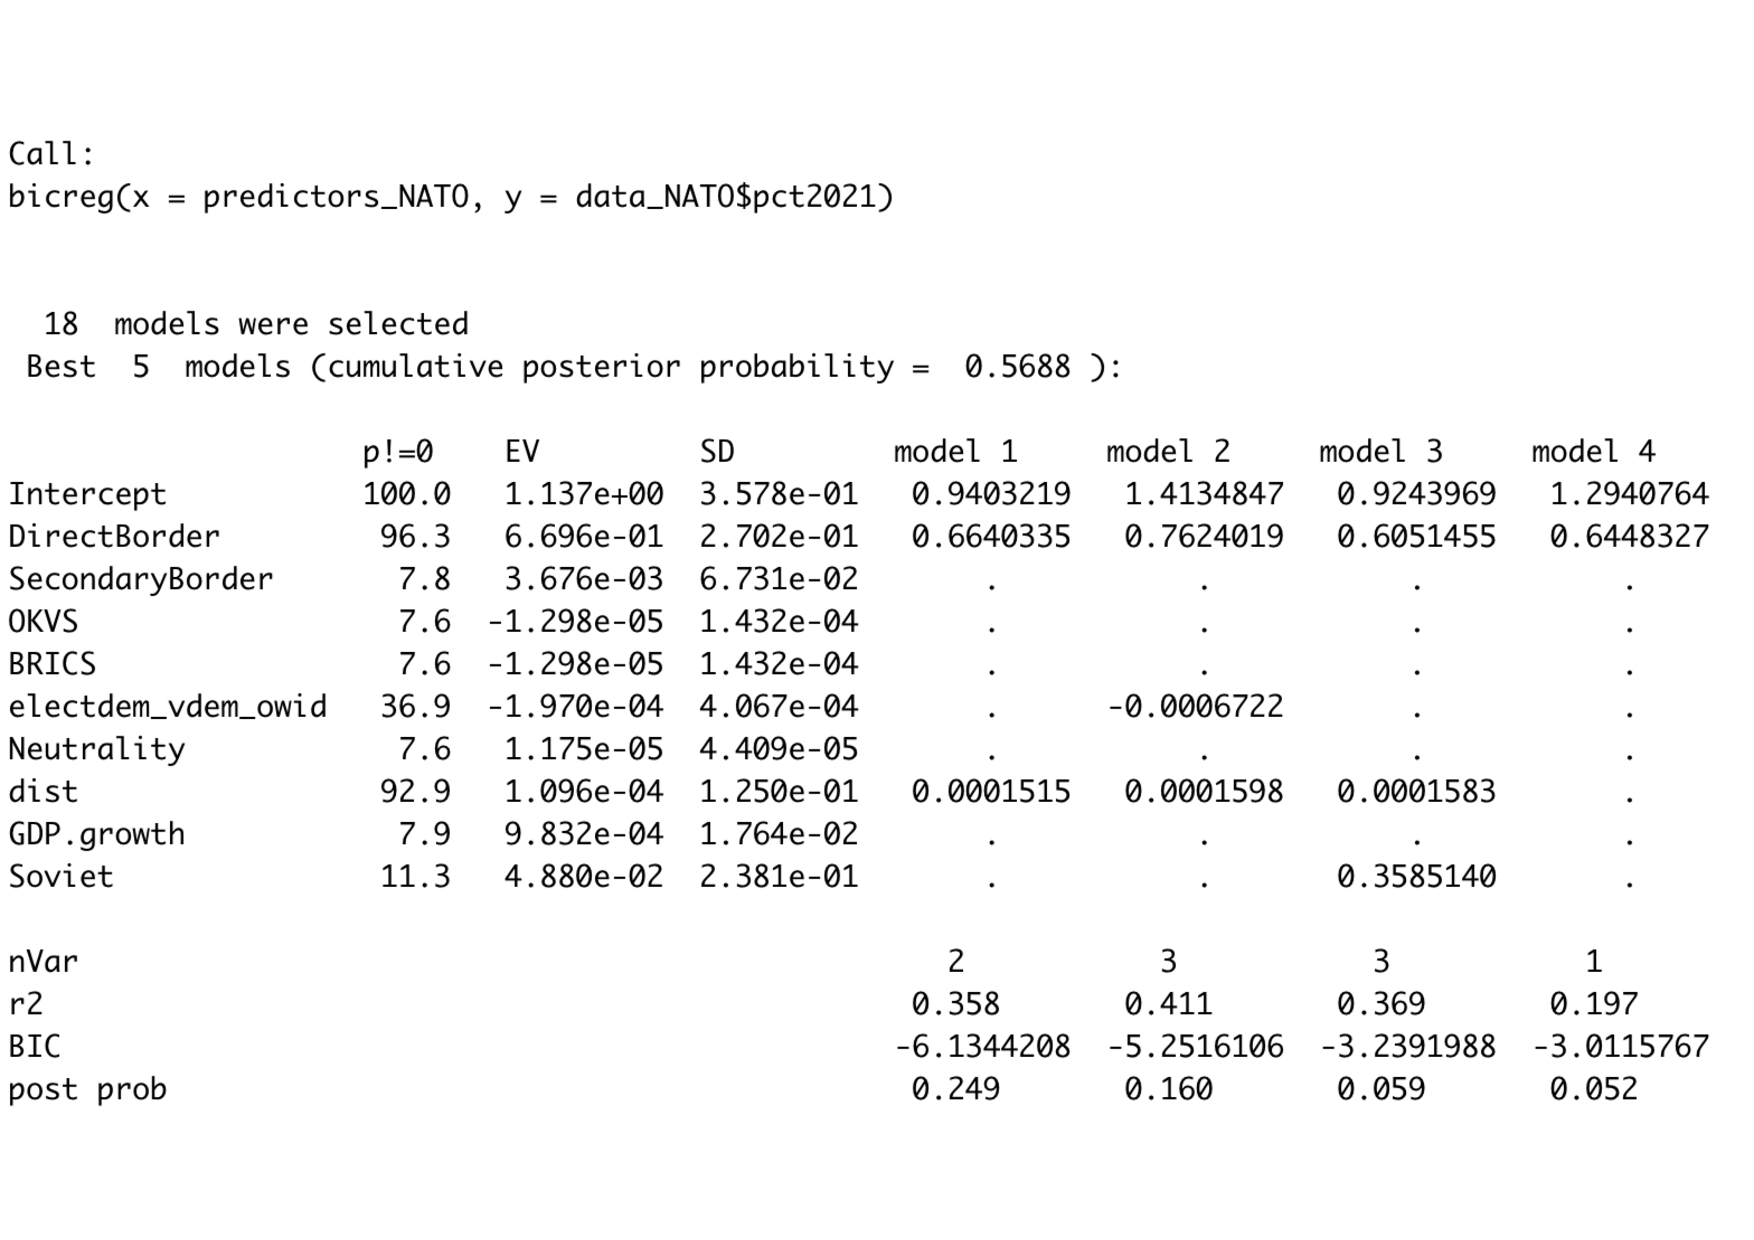
\includegraphics[scale=0.4]{BMA_NATO}
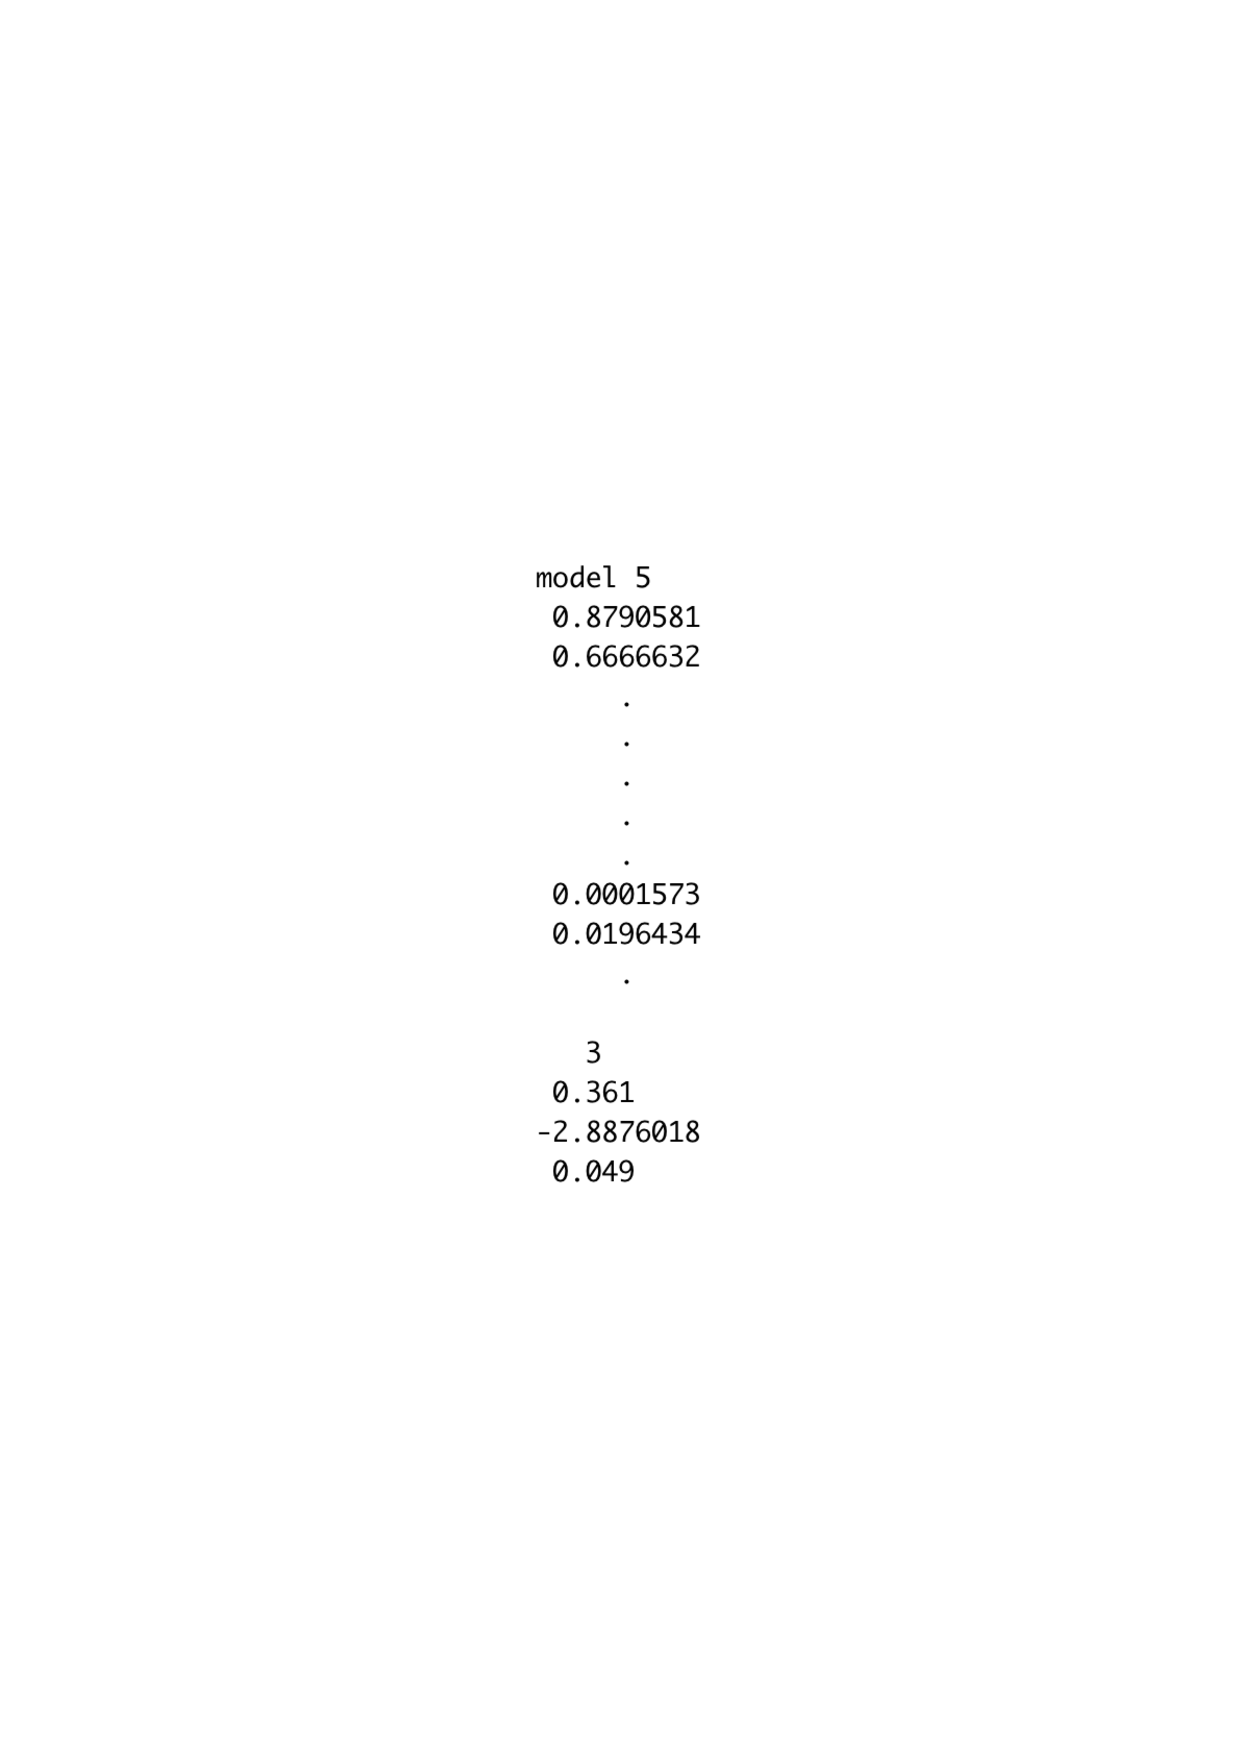
\includegraphics[scale=0.4]{BMA_NATO_2}
\caption{Bayesian Model Averaging - NATO members}
\end{figure}

When we narrow our focus to NATO member countries (see Figure 2), the results take on a different complexion. In this analysis, 18 models were generated, and the top five are presented here. Notably, in this Bayesian Model Averaging approach, the "Direct Border" variable assumes a pivotal role. It is included in all five of the suggested models and the coefficient has a probability of 96.3\% to be not zero among the 18 models generated, which deviates from the analysis of the entire dataset.

Additionally, the distance variable features in the first three suggested models and the coefficient has a probability of being not zero of 92.9\%, once again implying a correlation between military expenditure and proximity to Russia. This strenghten our core reserach hypothesis. In this specific analysis, the "V-Dem" variable assumes a lesser role, appearing only in the second model. What's noteworthy is the inclusion of the "GDP growth" variable in the fifth suggested model and the variable for a former member of the Soviet union in the third model, a new development compared to the previous analysis. Conversely, the variables "Secondary Border," "OKSV," and "BRICS" are once again absent in all of the models. \\


\subsection{EU members}
\begin{figure}[h]
\center
\label{F:1}
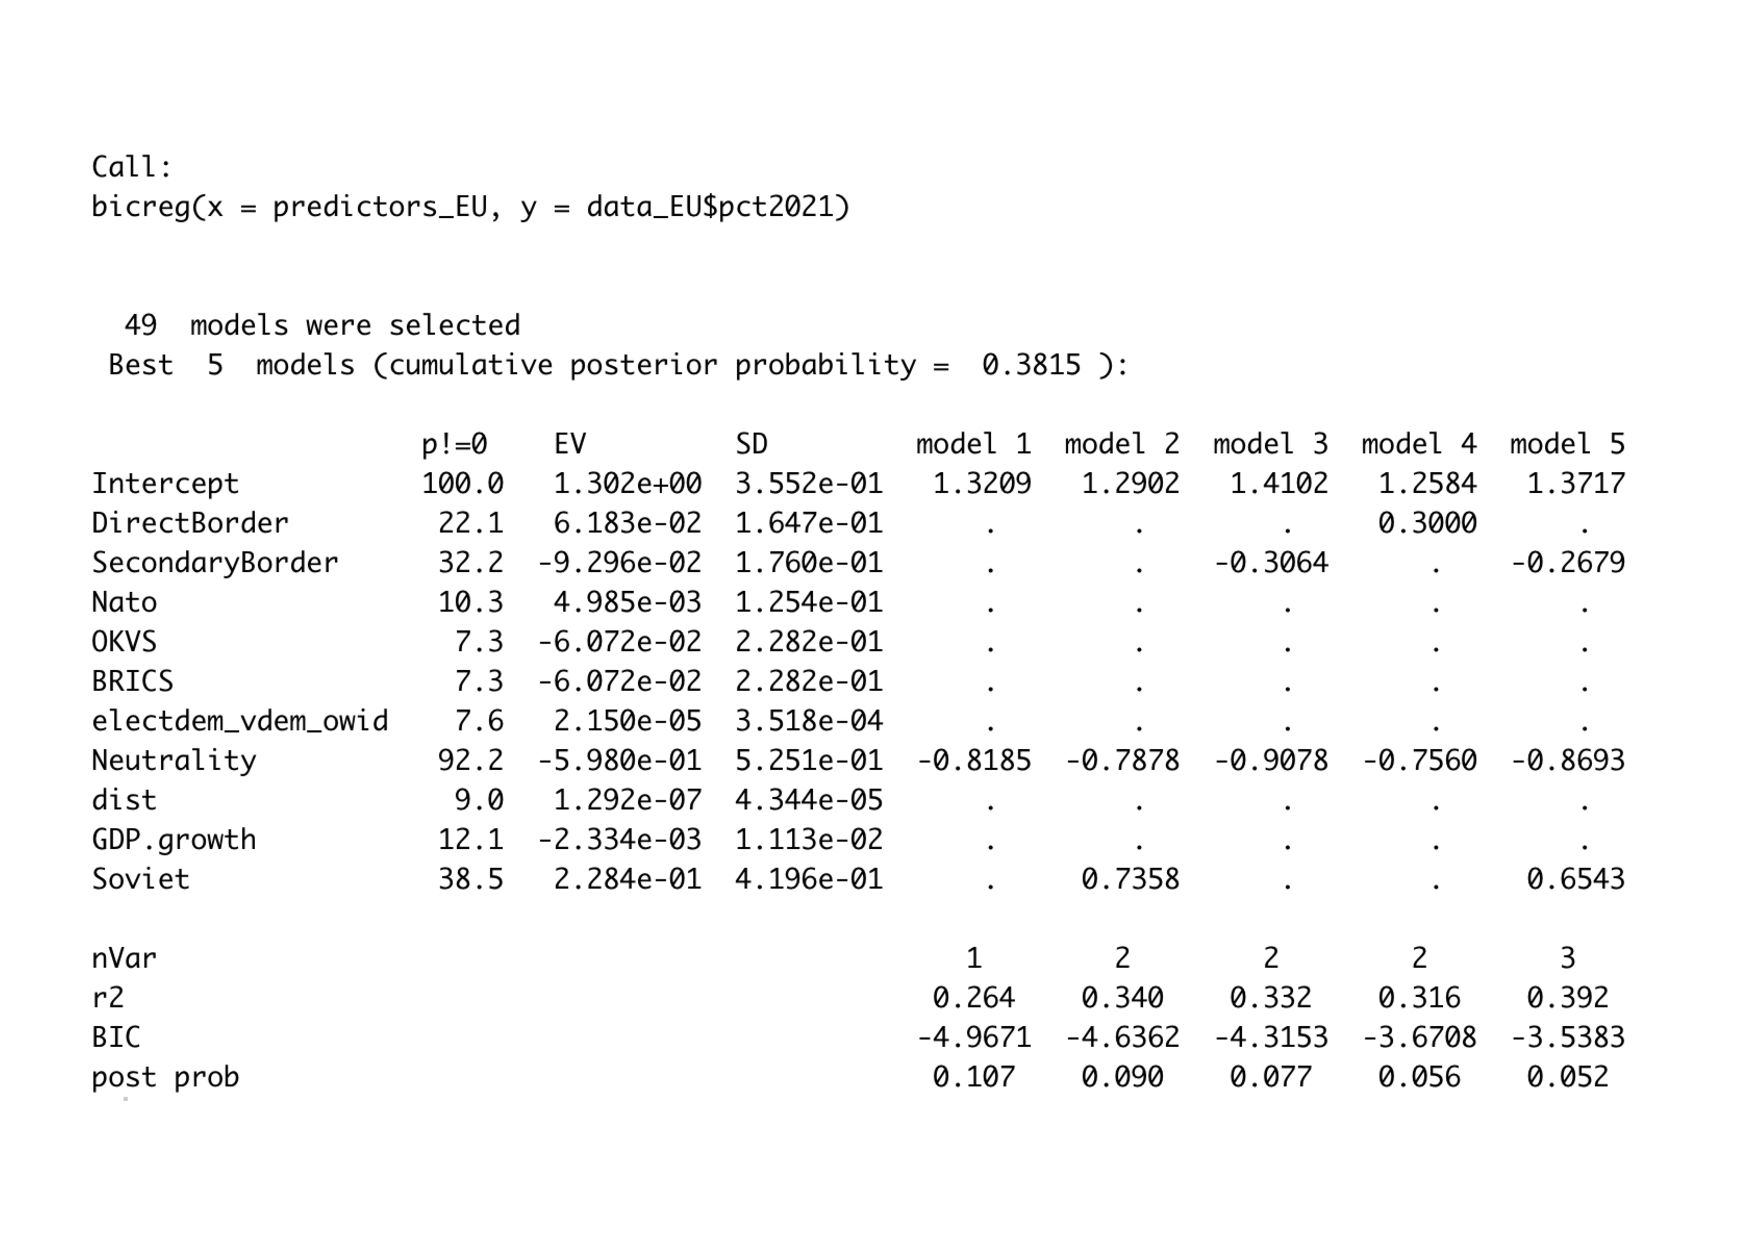
\includegraphics[scale=0.5]{BMA_EU}
\caption{Bayesian Model Averaging - EU members}
\end{figure}

Once again, focusing specifically on EU member countries (see Figure 3), yields markedly distinct results. Interestingly, the distance variable is absent from all of the suggested models in this context. Moreover, the probability that the coefficient for the predictor "dist" is non-zero among the 49 generated models is relatively low at 9\%. Instead, the "SecondaryBorder" variable makes an appearance in two of the five suggested models (32.2\% probability for the coefficient to be non-zero), while the "DirectBorder" variable features in one of them (22.1\% probability for the coefficient to be non-zero). The sudden transition from emphasizing the significance of the distance variable to highlighting the importance of the Border variables requires a potential interpretation. One possible explanation is that when the focus shifts to EU countries, the relevance of the air distance between a country's capital and Moscow diminishes. This is because EU capitals themselves are relatively close to each other compared to the global context. As a result, the significance of air distance decreases, and the direct or indirect exposure, as indicated by the Border dummy variables, assumes a more pivotal role. For instance, Baltic countries are directly exposed to Russia, potentially leading decision-makers to allocate a higher military expenditure compared to countries that do not share a direct or indirect border with Russia.

Notably, the variable that assumes the most significance in this Bayesian Model Averaging (BMA) analysis is "Neutrality," as it appears in all five suggested models and there is a high probability of 92.2\% that its coefficient is non-zero among the generated models. The first Model suggests, that a country claming itself as politically neutral will have a negative correlation with the military expenditure of that country (coefficient: -0.8185). Additionally, the "Soviet" variable is included in two of the suggested models with a positive coefficient and a relaitvely high probability for the coefficient to be non-zero among the estimated moderls with 38.5\%.  Both of these variables pertain to political relationships and the coefficients exhibit signs, which are in line with our expectations. None of the other variables are incorporated.


\section{Discussion}
\subsection{Implication}

In conclusion, based on the results presented above, it becomes evident that the composition of the dataset and, consequently, the countries under observation have a significant impact on the outcomes derived from BMA. Notably, the role of the distance variable varies across different analyses. 

In both the analysis of the entire dataset and the NATO subset, the distance variable assumes a crucial role, implying a correlation between military expenditure and proximity to Russia. However, this variable appears to have no relevance when examining EU countries, where the Direct and Secondary Border Variables seem to be influential instead.

Our core research question revolved around whether the geographical distance to Russia influences a country's decision-making regarding military expenditure. Our primary hypothesis stated that closer proximity to Russia would correlate positively with increased military expenditure by the respective country. By and large, we can conclude that our hypothesis has been suppoerted by our findings. \\

\subsection{Limitations}
In drawing these conclusions, we anticipate that our paper is subject to several limitations that could be addressed by further research. One such limitation pertains to the choice of control variables we employed.

Given that the BMA approach aims to identify the "best" model, a more extensive inclusion of variables could enhance the robustness and validity of the models. In particular, a more comprehensive consideration of distance-related variables might have further refined our results. For instance, Kofron and Stauber (2023) included not only Road Travel Distance and Flight Distance from capital to capital but also "the Square-rooted road travel distance between the nearest Russian military brigade-sized base and the nearest regional administrative center on the side of analyzed states." Furthermore, we did not incorporate variables that represent a country's internal security, unlike Nordhaus et al. (2012), who integrated variables such as the weighted military expenditures of friendly and hostile nations and the estimated annual probability of a significant civil conflict. Kofron and Stauber (2023) also considered factors like the number of terrorist attacks within a country. Additionally, we did not control for ongoing civil wars within these countries or conflicts with other nations, such as the Azerbaijan-Armenia conflict. Another limitation lies in our use of dummy variables to capture the political orientation of a government. Kofron and Stauber (2023) employed a more detailed measure, "The proportion of representation of political parties classified as social democratic," which could potentially provide a more nuanced understanding than our simplistic "BRICS" dummy. To comprehensively address the multifaceted factors influencing military expenditure, further research could explore additional variables encompassing economic, political, and strategic dimensions, as suggested by Nikolaidou (2008).\\

Furthermore, it's important to acknowledge that our chosen method comes with certain limitations. When examining the R packages we utilized, we find that there are several alternatives available, some of which could have provided greater flexibility in selecting specific features. For instance, the BMS and BAS packages offer considerable freedom in terms of choosing model priors and priors for the regression coefficients (Amini and Parmeter, 2011). This increased flexibility would have enabled us to run the analysis with different priors and compare the resulting outputs. Additionally, our decision to conduct a cross-sectional analysis for only one year, rather than considering multiple years or employing a time-series analysis, means that we were unable to account for changes over time. Military expenditure in a country can be influenced by its own historical spending patterns, and a Vector Autoregressive Analysis might have revealed valuable insights in this regard. \\

Additionally, we do not fully explore the possibility of using more flexible models, such as generalized additive models or Bayesian additive regression trees, which may better fit the data and reveal more complex relationships. Especially spatial models could have accounted for the spatial dependence or heterogeneity of military expenditures across countries. This might have improved our model as we migth have ignored a triangular correlation between continent, geographic and cultural distance. Spatial models, hence, would have offered a more realistic and flexible way to model the underlying spatial autocorrelation and heterogeneity.\\

Finally, the choice of data may lead to validity problems. Besides to already mentioned limitation of generalization w.r.t. time and the possible bias w.r.t. to the used electoral democracy index, especially the SIRPI database could induce validity problems, which we are not able to control for. Although the SIRPI tries to use as few secondary sources in form of estimates as possible and to validate these in retrospect, it is nevertheless necessary for us to rely completely on the data generation process. This reliability, however, is questionable, especially in terms of military data and the strategic communication of the latter. On the one hand, it may be possible that deliberate information on military spending is being whitewashed; on the other hand, a ''filter bubble bias'' could arise if the data is based on estimates that include the same covariates as we include to explain variation. A next step would be to verify our results with similar datasets, e.g. the Correlates of War (CoW) dataset.


\section{Conclusion}
Our research project contributes to the existing literature by focusing on the geographical distance to Russia as a key determinant of military spending. The novel approach in this research area of employing Bayesian Model averaging offers a robust econometric method for analyzing complex relationships that demand a high number of control variables and could be extended to further research on military expenditures. 
While our project provides evidence in favor of geographical distance to a possible threat being one determining factor of military expenditures, there are still several avenues for further explorations. Investigating the reasons behind specific countries’ deviations from the 2 \% GDP allocation norm within NATO and understanding how regional alliances or geopolitical interests might interact with geopolitical proximity could yield additional valuable findings. 

By utilizing measures beyond just capital city distances as a proxy for distance, our analysis reveals diverse results prompting us to consider whether further exploration with different distance definitions could contribute further to understanding this area. Moreover, a potential shift from geographical distance to political distance to Russia could still provide a fresh perspective, exploring, how countries’ political perception of Russia influences their defense spending over time.

In conclusion, our research underscores the importance of physical geography and external security factors influencing military spending decisions. By examining the influence of geographical distance to Russia on military expenditures, we have enriched our understanding of how perceived threats and security concerns are translated into defense policies on a global scale. The finding from our analysis suggest that Policymakers should consider the geographical context and security concerns when allocating defense budgets and contribute to the broader discourse on defense spending determinants, encouraging further exploration in this area.  




\clearpage


%------------------------------------------------------------------%
\section{References}
Albalate, D., Bel, G. and Elias, F., 2012. Institutional determinants of military spending. Journal of comparative economics, 40(2), pp.279-290. \\

Amini, S.M. and Parmeter, C.F., 2011. Bayesian model averaging in R. Journal of Economic and Social Measurement, 36(4), pp.253-287. \\

Brown, P.J., Vannucci, M. and Fearn, T., 2002. Bayes model averaging with selection of regressors. Journal of the Royal Statistical Society Series B: Statistical Methodology, 64(3), pp.519-536.\\

Buch, C.M., 2005. Distance and international banking. Review of International Economics, 13(4), pp.787-804. \\

Clyde, M. and George, E.I., 2004. Model uncertainty.\\

Coppedge, M., Gerring, J., Knutsen, C. H., Lindberg, S. I., Teorell, J., Altman, D., Bernhard, M., Cornell, A., Fish, M. S., Gastaldi, L., Gjerloew, H., Glynn, A., God, A. G., Grahn, S., Hicken, A., Kinzelbach, K., Krusell, J., Marquardt, K. L., Mc- Mann, K., Mechkova, V., Medzihorsky, J., Natsika, N., Neundorf, A., Paxton, P., amd Josefine Pernes, D. P., Ryden, O., von Roemer, J., Seim, B., Sigman, R., Skaaning, S.-E., Staton, J., Sundstroem, A., Tzelgov, E., ting Wang, Y., Wig, T., Wilson, S., and Ziblatt, D. (2023). ”v-dem [country-year/country-date] dataset v13” varieties of democracy (v-dem) project. https://doi.org/10.23696/vdemds23. \\

Dunne, J.P. and Perlo-Freeman, S., 2003a. The demand for military spending in developing countries: A dynamic panel analysis. Defence and Peace Economics, 14(6), pp.461-474.\\

Dunne, P. and Perlo-Freeman, S., 2003b. The demand for military spending in developing countries. International Review of Applied Economics, 17(1), pp.23-48. \\

George, J. and Sandler, T. (2018). Demand for military spending in nato, 1968–2015: A spatial panel approach. European Journal of Political Economy, 53:222–236. \\

Gray, C. S. (2005). How has war changed since the end of the cold war? The US Army War College Quarterly: Parameters, 35(1):7. \\

Hoeting, J.A., Madigan, D., Raftery, A.E. and Volinsky, C.T., 1999. Bayesian model averaging: a tutorial (with comments by M. Clyde, David Draper and EI George, and a rejoinder by the authors. Statistical science, 14(4), pp.382-417. \\

Jeffreys, H. (1939). The theory of probability. Oxford University Press., Oxford, England, 1 edition. \\

Jevons, W. S. (1874). The mathematical theory of political economy. Journal of the Royal Statistical Society Series A: Statistics in Society, 37(4):478–488. \\

Kofron, J. and Stauber, J. (2023). The impact of the russo-ukrainian conflict on mil- itary expenditures of european states: security alliances or geography? Journal of Contemporary European Studies, 31(1):151–168. \\

Lin, F.L. and Wang, M.C., (2019). Does economic growth cause military expenditure to go up? Using MF-VAR model. Quality \& Quantity, 53, pp.3097-3117. \\

Moral‐Benito, E., 2015. Model averaging in economics: An overview. Journal of Economic Surveys, 29(1), pp.46-75.\\

Mayer, T. and Zignago, S. (2011). Notes on cepii’s distances measures: The geodist database. CEPII working paper.\\

Nikolaidou, E., 2008. The demand for military expenditure: Evidence from the EU15 (1961–2005). Defence and Peace Economics, 19(4), pp.273-292.\\

Starkweather, J., 2011. Sharpening Occam’s Razor: Using Bayesian Model Averaging in R to Separate the Wheat from the Chaff. Benchmarks RSS Matters. Retrieved online, 5, p.13.\\

Steel, M.F., 2020. Model averaging and its use in economics. Journal of Economic Literature, 58(3), pp.644-719.\\

Mayer, T. and Zignago, S. (2011). Notes on cepii’s distances measures: The geodist database. CEPII working paper. \\

Nikolaidou, E. (2008). The demand for military expenditure: Evidence from the eu15 (1961–2005). Defence and Peace Economics, 19(4):273–292. \\

Nordhaus, W., Oneal, J. R., and Russett, B. (2012). The effects of the international security environment on national military expenditures: A multicountry study. Inter- national Organization, 66(3):491–513. \\

Odehnal, J. and Neubauer, J. (2020). Economic, security, and political determinants of military spending in nato countries. Defence and Peace Economics, 31(5):517–531. \\

SIPRI Military Expenditure Database (2023). https://www.sipri.org/databases/ milex. \\

Watanabe, S. (2010). Asymptotic equivalence of bayes cross validation and widely ap- plicable information criterion in singular learning theory. Journal of machine learning research, 11(116):3571–3594. \\

World population review, https://worldpopulationreview.com/country-rankings/neutral-countries \\



\end{document}
